\section{Kolmogorov's Big Measure: How Probability Went From Dice Rolls to Digital Revolution (1933)}

\subsection{Kolmogorov's Big Idea: Measure Everything}

Before the 20th century, probability theory was basically just glorified dice rolling. However, the moment probability needed to handle continuous random variables, stochastic processes, and the horrifying abyss of infinity, classical methods broke down. 

This is where \textbf{Andrey Kolmogorov} enters the chat. 

Kolmogorov did what mathematicians do best when the world refuses to behave: he gave it an axiomatic framework and dared anyone to object. His key move? He redefined probability to be about it was about measuring space using the same mathematical machinery that Lebesgue had invented for measuring strange, fragmented, or downright pathological sets.

Imagine a vast landscape and call it your "sample space" \( \Omega \). Now, highlight a region \( A \subset \Omega \), like "everywhere the delivery robot could crash" or "the area where the experiment might explode." Kolmogorov says: \textbf{Don’t count outcomes; \textit{Measure} the size of that set}. 

With this insight, we get:

\[
P(A) = \text{measure of } A
\]

Where \( A \) is a measurable subset of the sample space: some region carved out of the universal possibility grid. 

\begin{figure}[H]
\centering
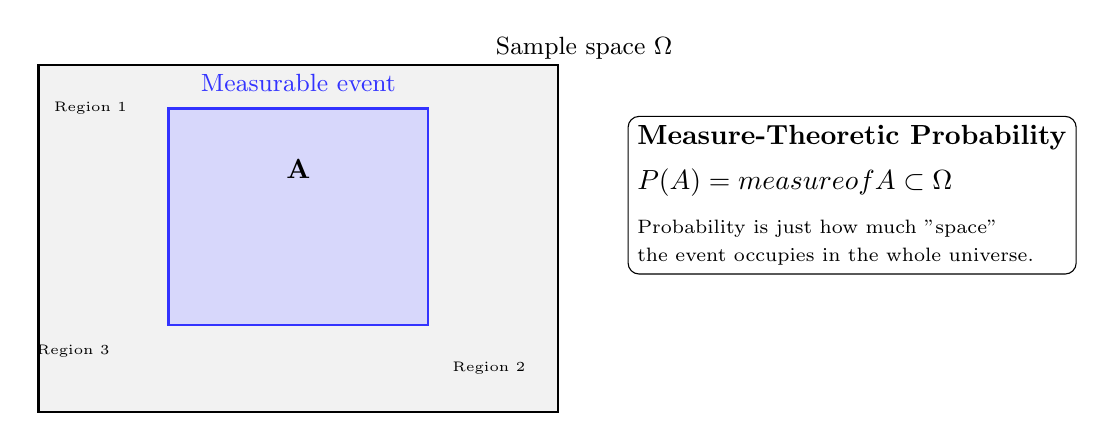
\begin{tikzpicture}[scale=1.1]

% Background rectangle representing sample space
\fill[gray!10] (-3,-2) rectangle (3,2);
\draw[thick] (-3,-2) rectangle (3,2);
\node at (3.3,2.2) {\small Sample space \( \Omega \)};

% Subset A (event of interest)
\fill[blue!20, opacity=0.7] (-1.5,-1) rectangle (1.5,1.5);
\draw[blue!80, thick] (-1.5,-1) rectangle (1.5,1.5);
\node at (0,0.8) {\textbf{A}};
\node[blue!80] at (0,1.8) {\small Measurable event};

% Text box
\node[draw, fill=white, rounded corners, align=left, anchor=west] at (3.8,0.5) {
\textbf{Measure-Theoretic Probability} \\[4pt]
\( P(A) = \text{measure of } A \subset \Omega \) \\[4pt]
\scriptsize Probability is just how much "space" \\[-2pt]
\scriptsize the event occupies in the whole universe.
};

% Some labels on the background
\node at (-2.4,1.5) {\tiny Region 1};
\node at (2.2,-1.5) {\tiny Region 2};
\node at (-2.6,-1.3) {\tiny Region 3};

\end{tikzpicture}
\caption{Kolmogorov’s view: probability as the area (measure) of a subset \( A \) inside the total sample space \( \Omega \). No counting. Just geometry.}
\end{figure}


Suddenly, everything becomes gloriously geometric:
\begin{itemize}
    \item The probability of hitting two regions at once? Take the intersection of their areas.
    \item The chance of one event given another? Divide the measures.
    \item The probability of either event happening (but not both)? Add their areas and subtract the overlap—like you’re doing union with a vengeance.
\end{itemize}

This measure-theoretic view let probability theory grow up. It could now handle continuous distributions, infinite sample spaces, and stochastic processes without breaking into hives.


But Kolmogorov didn’t stop there—he also untangled one of the most frustrating paradoxes in geometric probability: the \textbf{Rotating Roulette Problem}.

Imagine this: You’ve got a perfect, frictionless roulette wheel, and you're dropping a grain of sand from the air. The sand lands randomly somewhere on the wheel’s surface. So far, so good.

Now ask: what’s the probability that the sand lands along a particular circular groove carved into the wheel?

You might think: “Well, any groove is just as good as another. So the chance should be evenly spread out across all grooves, right?”

Not quite.

If you consider concentric grooves (like rings), the sand is more likely to hit the outer ones than the inner ones. Why? Because they cover more surface area. But if you rotate the wheel, those outer grooves become vertical ones—and now the probabilities aren’t uniform anymore. It feels like cheating.

Kolmogorov resolved the paradox by showing that these grooves are one-dimensional slices through a two-dimensional space. And one-dimensional slices in a two-dimensional space have \textbf{measure zero}. You can’t meaningfully assign a probability to the sand hitting a specific groove—because grooves, like great circles on a sphere, take up no area.



\begin{figure}[H]
\centering
\begin{tikzpicture}[scale=1.1]

% ---------- Top panel: geometric probability ----------
% Background rectangle
\fill[gray!10] (-3,-2) rectangle (3,2);
\draw[thick] (-3,-2) rectangle (3,2);

% Region A
\fill[blue!20] (-2.2,-0.5) rectangle (0.3,1.2);
\draw[blue!80, thick] (-2.2,-0.5) rectangle (0.3,1.2);
\node at (-1.0,1.3) {\small Event A};

% Region B
\fill[red!20] (-0.3,-1.2) rectangle (2.0,0.5);
\draw[red!80, thick] (-0.3,-1.2) rectangle (2.0,0.5);
\node at (1.1,-1.3) {\small Event B};

% Intersection
\fill[blue!50,opacity=0.5] (-0.3,-0.5) rectangle (0.3,0.5);

% Sample space label (below the rectangle)
\node at (0,-2.4) {\small Sample space \( \Omega \)};

% Equation block (centered vertically with rectangle)
\node[align=left] at (6.4,0) {
    \small \textbf{Measure-Theoretic Rules:} \\[4pt]
    \( P(A \cap B) \) -- both happen \\[2pt]
    \( P(A \cup B) = P(A) + P(B) - P(A \cap B) \) \\[2pt]
    \( P(A|B) = \dfrac{P(A \cap B)}{P(B)} \)
};

% Divider line
\draw[dashed, thick] (-3.5,-2.8) -- (7.0,-2.8);

% ---------- Bottom panel: roulette paradox ----------
\begin{scope}[shift={(0,-6.5)}]
    \shade[ball color=gray!15] (0,0) circle (2);
    \draw[thick] (0,0) circle (2);
    \draw[thick, red!70] (0,0) circle (0.4);
    \draw[thick, red!70] (0,0) circle (1.2);

    % Grain of sand
    \filldraw[black] (1.3,0.5) circle (1.2pt);

    % Grain of sand label with arrow stopping before the point
    \node at (2.6,1.2) {\tiny Grain of sand};
    \draw[->, thick] (2.4,1.1) -- (1.45,0.65); % stops just before the actual grain

    % Groove label at top of circle
    \node[red!70] at (0,2.2) {\tiny Concentric groove};
    \draw[->, red!70] (0,2.1) -- (0,1.3);

    % Equation box for measure zero (right)
    \node[align=left] at (6.4,0.6) {
        \small \textbf{Roulette Paradox:} \\[4pt]
        Grooves are 1D curves in 2D \\[-2pt]
        \( \Rightarrow \text{Area} = 0 \) \\[2pt]
        \( \Rightarrow P(\text{hit groove}) = 0 \)
    };

    \node at (0,-2.4) {\small Roulette wheel with grooves};
\end{scope}

\end{tikzpicture}
\caption{Top: Kolmogorov’s view of probability as area—intersections, unions, and conditional probability as geometric operations. Bottom: In the rotating roulette paradox, grooves have measure zero, so hitting one has zero probability.}
\end{figure}




The problem wasn’t in the math. The problem was in the question.

Kolmogorov’s real gift wasn’t just giving probability a rigorous foundation—it was giving us a way to know when our intuitions were lying to us.

Which, as it turns out, they usually are.


\subsection{Kolmogorov’s Axioms: When Probability Found Religion}

In the previous section, we saw how Kolmogorov reimagined probability through the lens of Lebesgue’s measure theory. He didn’t care how many darts you threw or how many roulette grooves you counted—he cared about how much measurable “space” your events occupied.

But this reinterpretation needed structure. So in 1933, Kolmogorov formalized the entire theory with a small but mighty set of axioms—rules so fundamental, they turned probability into a full-fledged branch of analysis.

You can think of these axioms as the laws that govern dart-throwing in infinite sample spaces:

\begin{enumerate}
    \item \textbf{Non-negativity:} \( P(A) \geq 0 \)  
    No negative probabilities—because what even is “negative chance”?

    \item \textbf{Normalization:} \( P(\Omega) = 1 \)  
    The probability that \emph{something} happens is 100\%. The dart always hits \emph{somewhere} on the board.

    \item \textbf{Countable Additivity:}  
    For any countable sequence of disjoint events \( A_1, A_2, A_3, \dots \),
    \[
    P\left(\bigcup_{i=1}^{\infty} A_i\right) = \sum_{i=1}^{\infty} P(A_i)
    \]
    This says: if no two regions overlap, just add up their areas—whether you’re dealing with three events or three hundred trillion.
\end{enumerate}




\begin{figure}[H]
\centering
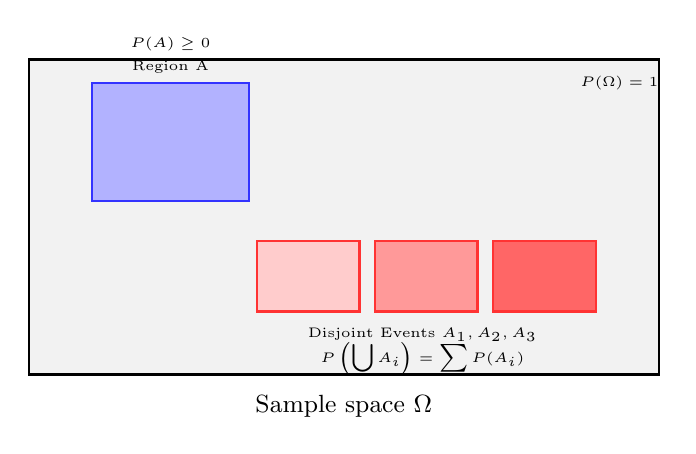
\begin{tikzpicture}[scale=1]

% Base rectangle (sample space)
\fill[gray!10] (-4,-2) rectangle (4,2);
\draw[thick] (-4,-2) rectangle (4,2);
\node at (0,-2.4) {\small Sample space \( \Omega \)};

% Region A for non-negativity (centered left)
\fill[blue!30] (-3.2,0.2) rectangle (-1.2,1.7);
\draw[blue!80, thick] (-3.2,0.2) rectangle (-1.2,1.7);
\node at (-2.2,1.9) {\tiny Region A};
\node at (-2.2,2.2) {\tiny \( P(A) \geq 0 \)};

% Disjoint events A1, A2, A3 (centered right)
\fill[red!20] (-1.1,-1.2) rectangle (0.2,-0.3);
\fill[red!40] (0.4,-1.2) rectangle (1.7,-0.3);
\fill[red!60] (1.9,-1.2) rectangle (3.2,-0.3);
\draw[red!80, thick] (-1.1,-1.2) rectangle (0.2,-0.3);
\draw[red!80, thick] (0.4,-1.2) rectangle (1.7,-0.3);
\draw[red!80, thick] (1.9,-1.2) rectangle (3.2,-0.3);

\node at (1.0,-1.5) {\tiny Disjoint Events \( A_1, A_2, A_3 \)};
\node at (1.0,-1.8) {\tiny \( P\left(\bigcup A_i\right) = \sum P(A_i) \)};

% Full space label for normalization
\node at (3.5,1.7) {\tiny \( P(\Omega) = 1 \)};

\end{tikzpicture}
\caption{Kolmogorov’s axioms in action: Probabilities are non-negative, the entire space has measure 1, and disjoint areas add up like Lego bricks.}
\end{figure}





\subsection{How Soviet Ideology Held Back the Digital Revolution}

The world finally had a rigorous foundation for probability. Mathematicians rejoiced. Soviet military strategists, however? They saw something very different.  You see, \textbf{probability isn’t just good for modeling dice rolls. It’s also good for, say… targeting artillery.}

During WWII, the Soviet military quickly realized that Kolmogorov’s work could make their artillery more accurate. The problem with traditional artillery calculations was that battlefield conditions are, well, chaotic: wind, terrain, and human error all make direct aim unreliable. But Kolmogorov’s measure-theoretic probability framework allowed them to model these uncertainties, improving Soviet targeting systems.  

And guess who took notice? \textbf{The RAND Corporation.}

Yes, the U.S. government’s premier think tank took a long, hard look at everything Kolmogorov was doing and said, “We’ll take that.” In classic American fashion, they stole his work, reverse-engineered them, and applied them to everything from missile guidance to financial models.

Meanwhile, the Soviets had one of the greatest mathematical minds in history, and then completely failed to capitalize on it.

Here’s the part where Soviet ideology shoots itself in the foot. You see, in addition to revolutionizing probability theory, Kolmogorov also did foundational work in information theory: the very field that would go on to power modern computers, cryptography, and artificial intelligence. 

But there was just one problem: \textbf{The Soviets thought digital technology was "capitalist."}  

I am not making this up. While the West was investing in digital computation, error correction, and cryptographic systems based on Kolmogorov’s work, the Soviet Union decided to stick with analog technology because digital systems were seen as a "capitalist tool of imperialism." 

Yes, that’s right. They had one of the greatest mathematicians of the 20th century literally laying out the blueprint for the information age, and they ignored him because of political ideology.  

\begin{tcolorbox}[colback=gray!5!white, colframe=black!80!white, title={Historical Sidenote: Lenin, Stalin, and the Machinery of Revolutionary Consciousness}]
  \textbf{Vladimir Lenin} believed that the proletariat would not, on its own, develop revolutionary consciousness. Left to their own devices, workers might demand better wages or shorter hours—but not the overthrow of capitalism. To bridge this gap, Lenin proposed the concept of the \emph{vanguard party}: a disciplined group of politically advanced thinkers who could inject Marxist theory into the spontaneous struggles of workers.  
  
  For Lenin, class struggle was necessary but not sufficient. Revolution required \emph{direction}—the kind that could only come from theory sharpened into strategy.  
  
  \medskip
  
  \textbf{Joseph Stalin}, inheriting this framework, industrialized it—sometimes literally. Under his rule, revolutionary consciousness became not just a philosophical objective, but a mass production goal. Factories didn’t just make tractors; they made \textbf{ideological subjects}. Through education campaigns, purges, and rigid planning, Stalin sought to turn the chaotic energy of labor into a centralized engine of socialist transformation.  
  
  \medskip
  
  In both cases, consciousness wasn’t a side effect—it was an engineered outcome. Lenin wanted workers to understand history; Stalin wanted them to \emph{embody} it.
\end{tcolorbox}


\subsection{From Probability to Digital Computation: The Path They Should Have Taken}  

Before Kolmogorov, probability theory was stuck in the arcade—good enough for dice, cards, and insurance tables, but not ready to handle the continuous chaos of the real world. Why? Because it relied on this naïve formula for expected value:

\[
E[X] = \sum_{i} x_i P(X = x_i)
\]

This is fine if you’re working with discrete variables, like counting how often a sensor outputs a voltage of exactly 1.5V or 3V. But try applying that to an analog microphone recording ambient noise, where voltage varies smoothly—good luck summing over infinite possibilities, each with probability zero.

Let’s walk through this.

Suppose a legacy sensor can only read voltages at fixed levels:  
\( x_1 = 0\text{V}, x_2 = 1\text{V}, x_3 = 2\text{V} \),  
with corresponding probabilities \( P(X = x_1) = 0.2, P(X = x_2) = 0.5, P(X = x_3) = 0.3 \).  
Then the expected voltage is:

\[
E[X] = 0 \cdot 0.2 + 1 \cdot 0.5 + 2 \cdot 0.3 = 1.1 \text{ V}
\]

Now consider a modern microphone producing a continuous range of voltages, say from 0V to 3V. Assume the noise follows a probability density function:

\[
f(x) = \frac{2}{9}(3 - x), \quad \text{for } x \in [0, 3]
\]

This is a triangular distribution skewed toward lower voltages. The expected value is:

\[
E[X] = \int_0^3 x f(x)\,dx = \int_0^3 x \cdot \frac{2}{9}(3 - x)\,dx
\]

Compute it:

\[
E[X] = \frac{2}{9} \int_0^3 (3x - x^2)\,dx = \frac{2}{9} \left[ \frac{3x^2}{2} - \frac{x^3}{3} \right]_0^3 = \frac{2}{9} \left( \frac{27}{2} - 9 \right) = \frac{2}{9} \cdot \frac{9}{2} = 1 \text{ V}
\]

So the expected voltage of the analog mic is 1V—slightly lower than the discrete case. Kolmogorov’s formulation lets us make this kind of precise statement, because it doesn’t require that outcomes be countable—it just requires that they be measurable.

\textbf{This is what turned probability into an analytic tool}. With measure-theoretic probability, we can now model noise, signal reconstruction, and uncertainty with real mathematical rigor.


\begin{figure}[H]
\centering
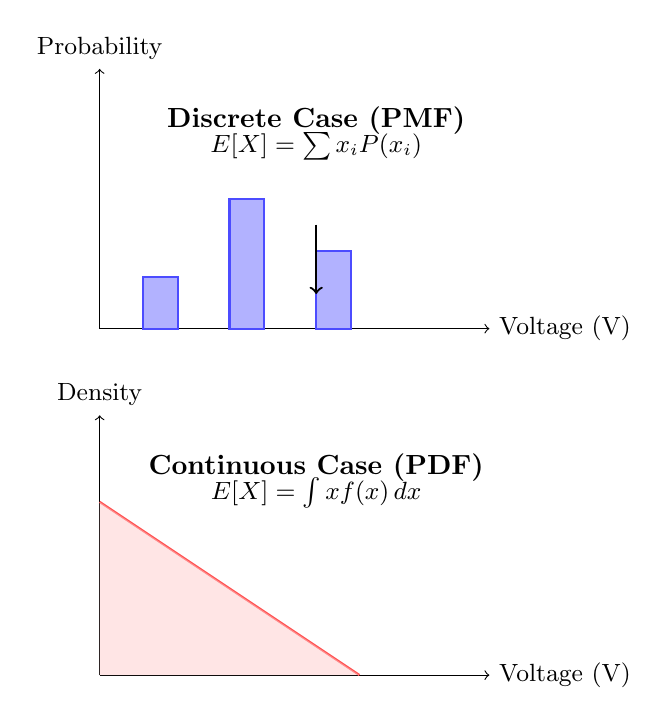
\begin{tikzpicture}[scale=1.1]

% Axes for discrete case
\draw[->] (0,0) -- (4.5,0) node[right] {\small Voltage (V)};
\draw[->] (0,0) -- (0,3) node[above] {\small Probability};

% Discrete bars (legacy sensor)
\foreach \x/\p in {0/0.6, 1/1.5, 2/0.9} {
    \draw[fill=blue!30, draw=blue!70, thick] (\x+0.5,0) rectangle (\x+0.9,\p);
}

\node at (2.5,2.4) {\textbf{Discrete Case (PMF)}};
\node at (2.5,2.1) {\small $E[X] = \sum x_i P(x_i)$};

% Arrow to continuous case
\draw[->, thick] (2.5,1.2) -- (2.5,0.4);

% Shift coordinate system down
\begin{scope}[shift={(0,-4)}]

% Axes for continuous case
\draw[->] (0,0) -- (4.5,0) node[right] {\small Voltage (V)};
\draw[->] (0,0) -- (0,3) node[above] {\small Density};

% PDF: f(x) = (2/9)(3 - x)
\draw[thick, red!70, domain=0:3, samples=100] plot (\x, {2*(3 - \x)/3});
\fill[red!20, opacity=0.5] (0,0) -- plot[domain=0:3, samples=100] (\x, {2*(3 - \x)/3}) -- (3,0) -- cycle;

\node at (2.5,2.4) {\textbf{Continuous Case (PDF)}};
\node at (2.5,2.1) {\small $E[X] = \int x f(x)\,dx$};

\end{scope}

\end{tikzpicture}

\vspace{1em}
\caption{Top: Discrete probability models voltage using countable values and finite sums. Bottom: Measure-theoretic probability uses density functions and integration to compute expectations over continuous distributions.}
\end{figure}

\subsection{From Voltages to Signals: Where Math Meets Time}

Once you can integrate a probability distribution over a continuous range, the natural next step is to ask: what if that “range” changes over time?

After all, the real world doesn’t give us one measurement—it gives us functions. A voltage that varies over time. A vibration across a bridge. A flickering signal from deep space. These are not static numbers—they’re waves, curves, data evolving through time.

But if probability theory now lives in the continuous world, thanks to Kolmogorov, so must our tools for analyzing these signals. That means we can’t just deal with isolated outcomes anymore—we need to integrate over entire functions.

Let’s say we’re observing a signal that varies continuously from 0 to 3 volts. We might model it using a probability density function:

\[
f(x) = \frac{2}{9}(3 - x), \quad \text{for } x \in [0, 3]
\]

This function tells us how likely we are to observe a voltage near a particular value. And if we want to know the expected voltage, we don’t sum—we integrate:

\[
E[X] = \int_0^3 x f(x)\,dx = \int_0^3 x \cdot \frac{2}{9}(3 - x)\,dx
\]

\[
= \frac{2}{9} \int_0^3 (3x - x^2)\,dx = \frac{2}{9} \left[ \frac{3x^2}{2} - \frac{x^3}{3} \right]_0^3 = 1 \text{ V}
\]

This framework lets us describe entire analog waveforms with mathematical precision.

But here's the twist: in practice, we never get the whole waveform. We sample it—at discrete points in time—and hope that’s enough to reconstruct the full signal.

That question—whether samples can faithfully preserve the original signal—will become very important later.

\begin{figure}[H]
\centering
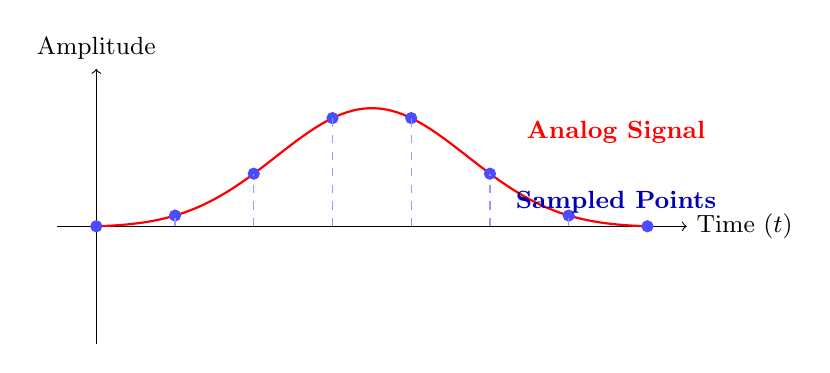
\begin{tikzpicture}[scale=1.0]

% Axes for top plot
\draw[->] (-0.5,0) -- (7.5,0) node[right] {\small Time ($t$)};
\draw[->] (0,-1.5) -- (0,2) node[above] {\small Amplitude};

% Continuous analog signal (smooth curve)
\draw[red, thick, domain=0:7, samples=100] plot(\x, {1.5 * sin(180 * \x / 7) * exp(-0.25*(\x - 3.5)^2)});
\node[red] at (6.6,1.2) {\small \textbf{Analog Signal}};

% Sampled points (blue dots)
\foreach \x in {0,1,2,3,4,5,6,7} {
    \filldraw[blue!70] (\x, {1.5 * sin(180 * \x / 7) * exp(-0.25*(\x - 3.5)^2)}) circle (2pt);
    \draw[blue!40, dashed] (\x,0) -- (\x, {1.5 * sin(180 * \x / 7) * exp(-0.25*(\x - 3.5)^2)});
}

\node[blue!70!black] at (6.6,0.3) {\small \textbf{Sampled Points}};

\end{tikzpicture}

\vspace{1em}
\caption{A continuous waveform and the samples we extract from it. Measure theory allows us to reason about the full analog signal—but soon, we’ll want to know how much is preserved in the samples alone.}
\end{figure}



\subsection{The Digital Divide: Mathematics Determines Technological Supe- riority}

Mathematically speaking, the Soviet Union had everything it needed to dominate the information age. They had Kolmogorov, the man who gave probability a foundation so strong that it eventually became the backbone of machine learning, digital signal processing, and high-frequency trading.

But there was just one problem: Soviet ideology was fundamentally deterministic.  

Marxist-Leninist philosophy viewed the universe as governed by strict laws—where everything, given enough knowledge, should be predictable. The idea that randomness was an inherent feature of nature? Unacceptable.

The moral of the story? \textbf{Mathematics determines who advances and who falls behind.}  

The West embraced probability and digital computation, while the Soviets clung to deterministic models, and that single decision changed the course of history.  

In the end, the most powerful weapon of the 20th century wasn’t the atomic bomb.  \textbf{It was math.}

\subsection{Ideology by Other Means: Mathematics and the Soviet Mind}

As the Soviet Union entered the postwar decades, mathematics became more than just a technical discipline—it became a terrain of ideological struggle. Andrey Kolmogorov, architect of modern probability and information theory, envisioned mathematics as a universal language, one that could rise above politics. In the 1960s, he spearheaded sweeping reforms to the Soviet school curriculum, embedding set theory, formal logic, and axiomatic structures at its core.\footnote{Kolmogorov’s reforms were implemented in the 1960s as part of the broader effort to modernize Soviet mathematics education. The new curriculum emphasized set theory, mappings, and abstract structures, and was codified in official state textbooks under his supervision. See Demidov, S.S., and Kolmogorov, A.N., \textit{Mathematics in the USSR}, Moscow, 1967.} His goal was not just pedagogy—it was protection. In a political climate where ideology dictated scientific truth, abstraction offered sanctuary. To teach students to think in terms of mappings, cardinalities, and logical implication was to equip them with habits of mind that could resist dogma.

But this quiet resistance drew fierce opposition. Lev Pontryagin—one of the USSR’s most decorated mathematicians and a war hero who had lost his sight as a teenager—saw Kolmogorov’s reforms as an elitist detour. To him, abstract set theory and logic had no place in the classroom of a socialist state. He dismissed the new curriculum as “bourgeois formalism,” detached from the material needs of Soviet society. In a widely circulated 1980 essay in \textit{The Communist}, the official journal of the Central Committee, Pontryagin and his colleagues warned that abstract mathematics was “alien to the Soviet spirit” and undermined the practical development of youth.\footnote{See L.S. Pontryagin, "On the Situation in the Teaching of Mathematics in Schools," \textit{The Communist}, No. 14 (1980), pp. 90–100. The article criticized the abstract orientation of mathematics education and explicitly targeted Kolmogorov’s reforms as elitist and ideologically misguided.}

This ideological shift had lasting consequences. By the late 1970s, Kolmogorov’s curriculum was dismantled, replaced with a more concrete, utilitarian approach. Geometry returned; logic disappeared. Mathematics was no longer a neutral zone—it had been reabsorbed into the ideological machinery of the Soviet state.

Ironically, it was Pontryagin’s own work that exemplified the union of mathematics and state power. His formulation of the \textbf{Pontryagin Maximum Principle} in 1956 provided the mathematical foundation for optimal control theory—a discipline born at the intersection of differential equations, variational calculus, and applied geometry. Control theory was not merely abstract—it was actionable. It allowed Soviet engineers and economists to design rockets, regulate power grids, and optimize production under constraint. Where Kolmogorov sought to insulate mathematics from ideology, Pontryagin’s legacy made it indispensable to the centralized logic of planning and control.

Thus, the tension between abstraction and application—between Kolmogorov’s probabilistic universality and Pontryagin’s geometric determinism—mirrored a deeper dialectic in Soviet intellectual life: the struggle over whether mathematics should transcend the state, or serve it.

\medskip

\begin{figure}[H]
\centering

% === First row ===
\begin{subfigure}[t]{0.45\textwidth}
\centering
\begin{tikzpicture}
  \comicpanel{0}{0}
    {Pontryagin}
    {}
    {\footnotesize He fills their heads with sets and symbols. They question geometry itself.}
    {(0,-0.6)}
\end{tikzpicture}
\caption*{The charge: corrupting young minds.}
\end{subfigure}
\hfill
\begin{subfigure}[t]{0.45\textwidth}
\centering
\begin{tikzpicture}
  \comicpanel{0}{0}
    {Party Official}
    {}
    {\footnotesize A bourgeois infection. Abstract thinking with no industrial use.}
    {(0,-0.6)}
\end{tikzpicture}
\caption*{The diagnosis: ideological abstractionitis.}
\end{subfigure}

\vspace{1em}

% === Second row ===
\begin{subfigure}[t]{0.45\textwidth}
\centering
\begin{tikzpicture}
  \comicpanel{0}{0}
    {Kolmogorov}
    {}
    {\footnotesize I only taught them to define a derivitive with epsilon and delta.}
    {(0,-0.6)}
\end{tikzpicture}
\caption*{The defense: precise definitions.}
\end{subfigure}
\hfill
\begin{subfigure}[t]{0.45\textwidth}
\centering
\begin{tikzpicture}
  \comicpanel{0}{0}
    {Soviet Tribunal}
    {}
    {\footnotesize Socrates corrupted the youth with logic, too.}
    {(0,-0.6)}
\end{tikzpicture}
\caption*{The sentence: curriculum rollback.}
\end{subfigure}

\caption{The Kolmogorov Trials: Where set theory met state theory.}
\end{figure}

